\chapter{Dynamic Equations}

In this chapter the forces and moments exerted on the aircraft will be presented. The main dynamic components are gravity, aerodynamic reactions and propulsion (also referred to as thrust).
\begin{equation}
	\bm{F}_b = \bm{F}_g + \bm{F}_a + \bm{F}_t
\end{equation}

\begin{lstlisting}
	F_x = F_g_x + F_a_x + F_t_x
	F_y = F_g_y + F_a_y + F_t_y
	F_z + F_g_z + F_a_z + F_t_z
\end{lstlisting}

Naturally, we consider that gravity does not exert moments on the rigid body aircraft.

\begin{equation}
	\bm{T}_b = \bm{T}_{a,tot} + \bm{T}_{t,tot}
\end{equation}

\begin{lstlisting}
	T_x = T_atot_x + T_ttot_x
	T_y = T_atot_y + T_ttot_y
	T_z = T_atot_z + T_ttot_z
\end{lstlisting}

Before proceeding to any definitions, it is worth mentioning the control input variables. In normal airplane configurations, there are four control dimensions which the pilot can affect. These correspond to three sets of control surfaces (aileron, elevator and rudder) and the throttle command. The notation for these control variables is $\delta_a, \delta_a, \delta_t, \delta_r$. Essentially, these are the input variables to the aircraft model.$\delta_a, \delta_e,$ and $\delta_r$ are usually expressed in degrees of deflection from the neutral (zero) angle and $\delta_t$ is normalized in the (0,1) range.

Conventions for the positive direction of each control surface are not always consistent. In this text, the proposed positive direction of a control surface is the one which results in a positive moment around each primary axis (aileron - roll right, elevator - pitch up, rudder - yaw right).

%% Gravity section
\section{Gravity}

Initially, we can assume a constant value for the acceleration of gravity, $g_0=9.805416m/s^2$ \cite[p.~8]{USStdAtm76}. The magnitude of the acceleration of gravity normally varies with altitude and geodetic coordinates, but a constant value is a valid approach for low altitude flight; unmodeled components are negligible to an adequate accuracy. If a more detailed gravity model is required (for example, in flights with vertical variance in the scale of kilometers), the reader can turn to Section \ref{sec:earth_model}. The orientation of the gravity vector is always vertical, towards the center of the Earth, thus in the z-direction in the NED frame.

\begin{equation} \label{eq:gravForce}
	\bm{F}_{g} = \bm{R}_b
	\begin{bmatrix}
		0\\ 0 \\mg
	\end{bmatrix}
\end{equation}
\begin{IEEEeqnarray}{rCl}
	{F}_{gx} &= &-\sin \theta ~m g \IEEEyessubnumber\\
	{F}_{gy} &= & \sin \phi \cos \theta ~m g  \IEEEyessubnumber\\
	{F}_{gz} &= & \cos \phi \cos \theta ~m g \IEEEyessubnumber
\end{IEEEeqnarray}

\begin{lstlisting}[style=C-style]
	F_g_x = -sin(theta)*m*g
	F_g_y = sin(phi)*cos(theta)*m*g
	F_g_z = cos(phi)*cos(theta)*m*g
\end{lstlisting}

\begin{equation}\label{eq:gravity}
	g = g_0
\end{equation}

%% Aerodynamics section 
\section{Aerodynamics}
This is the defining part of the flight characteristics of an airplane. The aerodynamic response of the airplane is crucial for its stability as well as its maneuverability.
Aerodynamic forces are presented in two frames of reference. The first is the body frame, whose corresponding forces, $\bm{F_a}$ are used for kinematic calculations. 
\begin{equation}
	\bm{F_a} = \begin{bmatrix}
	F_{ax} \\ F_{ay} \\ F_{az}
	\end{bmatrix}
\end{equation}
Aerodynamic forces are considered to be exerted, under normal operation, at the \emph{center of lift} ($\bm{p}_{CoL}$), a point located on the symmetry plane of the aircraft at one-quarter of the main wing chord.

However, for both historical and practical reasons, the flight characteristics of the airplane and the resulting forces (lift, drag and sideforce) are expressed in the stability frame (see \ref{eq:StabMatrix}). Models of aircraft aerodynamics are also parametrized so as to predict the aerodynamic forces in the stability frame as well.

\begin{equation}
	\bm{F_s} = \begin{bmatrix}
	-F_D \\ F_Y \\ -F_L
	\end{bmatrix}
\end{equation}

Thus, we can obtain $\bm{F}_a$ via the equation
\begin{equation}
	\bm{F}_a = \bm{S}^T \bm{F}_s
\end{equation}

We remind that
\begin{equation*}
	\bm{S} =
	\begin{bmatrix}
		\cos \alpha \cos \beta  & \sin \beta & \sin \alpha \cos \beta  \\
		-\cos \alpha \sin \beta & \cos \beta & -\sin \alpha \sin \beta \\
		-\sin \alpha            & 0          & \cos \alpha
	\end{bmatrix}
\end{equation*}

\begin{IEEEeqnarray}{rCl}
	F_{ax} &= & -\cos \alpha F_D -\cos \alpha \sin \beta F_Y + \sin \alpha F_L \IEEEyessubnumber\\
	F_{ay} &= & -\sin \beta F_D + \cos \beta F_Y \IEEEyessubnumber \\
	F_{az} &= & -\sin \alpha \cos \beta F_D -\sin \alpha \sin \beta F_Y - \cos \alpha F_L \IEEEyessubnumber
\end{IEEEeqnarray}

\begin{lstlisting}[style=C-style]
	F_a_x = -cos(alpha)*F_D - cos(alpha)*sin(beta)*F_Y + sin(alpha)*F_L
	F_a_y = -sin(beta)*F_D + cos(beta)*F_Y
	F_a_z = -sin(alpha)*cos(beta)*F_D - sin(alpha)*sin(beta)*F_Y - cos(alpha)*F_L
\end{lstlisting}

Aerodynamic moments need not be modeled in the stability frame. However, forces are generally not applied on the center of gravity of the aircraft, thus we need to model the moment they apply on it separately.
Sources of such additional moments are the stability margin (how much forward than the center of lift lies the center of mass), height difference between center of mass and center of lift (for example in a high-wing aircraft) and mass additions and subtractions to the airframe.

\begin{equation}
	\bm{T_{a,tot}} = \begin{bmatrix}
		T_{ax} \\ T_{ay} \\ T_{az}
		\end{bmatrix}
		+\left(\bm{p}_{CoL} - \bm{p}_{CG}\right) \times \bm{F}_a
\end{equation}
\begin{IEEEeqnarray}{rCl}
	T_{ax,tot} &= & T_{ax} -dz F_{ay} + dy F_{az}\IEEEyessubnumber\\
	T_{ay,tot} &= & T_{ay} +dz F_{ax} - dx F_{az}\IEEEyessubnumber\\
	T_{az,tot} &= & T_{az} -dy F_{ax} + dx F_{ay}\IEEEyessubnumber
\end{IEEEeqnarray}

\begin{lstlisting}[style=C-style]
	dx = p_cl_x - p_cm_x
	dy = p_cl_y - p_cm_y
	dz = p_cl_z - p_cm_z
	T_atot_x = T_a_x - dz*F_a_y + dy*F_a_z
	T_atot_y = T_a_y + dz*F_a_x - dx*F_a_z
	T_atot_z = T_a_z - dy*F_a_x + dx*F_a_y
\end{lstlisting}

The next step in exploring the aerodynamic model is the definition of dynamic pressure. This quantity expresses the pressure exerted by the air moving around the airplane per unit of surface. It is proportional with the density of the air and with the square of the airspeed. Dynamic pressure is a crucial scaling factor for the rest of the aerodynamic equations
\begin{equation}
	\bar{q} = \frac{1}{2}\rho V_a^2
\end{equation}

\begin{lstlisting}
	q_bar = 0.5*rho*V_a*V_a
\end{lstlisting}

The air density, $\rho$, is dependent upon altitude. Its sea level value ($\rho_0 = 1.225 kg/m^3$) is often used as an approximate value for low-altitude flight, but if needed, accurate atmospheric models are provided in Section \ref{sec:atm_model}.

We are now able to express the force components as the product of dynamic pressure, the wing surface $S$, and the aerodynamic coefficients of lift, drag and sideforce, $C_L$, $C_D$, $C_Y$. It is very important to appreciate that these coefficients are not constant values; instead, they are functions of the state of the flying body, albeit their dependence from some state variables is more dominant than others. A more detailed explanation is given further down.
\begin{IEEEeqnarray}{rCl}
	F_D &= &\bar{q} S C_D \IEEEyesnumber \IEEEyessubnumber \\
	F_Y &= &\bar{q} S C_Y \IEEEyessubnumber\\
	F_L &= &\bar{q} S C_L \IEEEyessubnumber
\end{IEEEeqnarray}

\begin{lstlisting}[style=C-style]
	F_D = q_bar*S*C_D
	F_Y = q_bar*S*C_Y
	F_L = q_bar*S*C_L
\end{lstlisting}

Generally, the aerodynamic coefficients are functions of the airspeed, aerodynamic angles, angular velocity and control inputs.

\begin{IEEEeqnarray}{rCl}
	C_D &= &C_D(V_a, \alpha, q, \delta_e) \IEEEyesnumber \IEEEyessubnumber \\
	C_Y &= &C_Y(V_a, \beta, p, r, \delta_a, \delta_r) \IEEEyessubnumber\\
	C_L &= &C_L(V_a, \alpha, q, \delta_e) \IEEEyessubnumber
\end{IEEEeqnarray}

The aerodynamic moments are defined in a similar fashion, with the additional inclusion of wingspan $b$ and wing chord $c$. The notation for the moment coefficients may vary from source to source.
\begin{IEEEeqnarray}{rCl}
	T_{ax} &= &\bar{q} S b C_l \IEEEyesnumber \IEEEyessubnumber \\
	T_{ay} &= &\bar{q} S c C_m \IEEEyessubnumber\\
	T_{az} &= &\bar{q} S b C_n \IEEEyessubnumber
\end{IEEEeqnarray}

\begin{lstlisting}[style=C-style]
	T_a_x = q_bar*S*b*C_l
	T_a_y = q_bar*S*c*C_m
	T_a_z = q_bar*S*b*C_n
\end{lstlisting}
%
\begin{IEEEeqnarray}{rCl}
	C_l &= &C_l(V_a, \beta, p, r, \delta_a, \delta_r) \IEEEyesnumber \IEEEyessubnumber \\
	C_m &= &C_m(V_a, \alpha, q, \delta_e) \IEEEyessubnumber\\
	C_n &= &C_n(V_a, \beta, p, r, \delta_a, \delta_r) \IEEEyessubnumber
\end{IEEEeqnarray}
%%
Finally, a model for the aerodynamic coefficients is provided. Undoubtedly, the most common and established approach is to use multivariable polynomials which are linear with respect to their coefficients. This representation lends itself nicely for parameter identification techniques, such as least-squares flavours, very common in real-world aircraft design and testing.
%
\begin{IEEEeqnarray}{rCl} \label{eq:forceCoeff} 
	C_D &=& C_{D,0} + C_{D,\alpha}\alpha+C_{D,q}\frac{c}{2V_a}q + C_{D,\delta_e}\delta_e \IEEEyesnumber \IEEEyessubnumber\\
	C_Y &=& C_{Y,0} + C_{Y,\beta}\beta + C_{Y,p}\frac{b}{2V_a}p + C_{Y,r}\frac{b}{2V_a}r + C_{Y,\delta_a}\delta_a + C_{Y,\delta_r}\delta_r \IEEEyessubnumber\\
	C_L &=& C_{L,0} + C_{L,\alpha}\alpha+C_{L,q}\frac{c}{2V_a}q +  C_{L,\delta_e}\delta_e \IEEEyessubnumber	
\end{IEEEeqnarray}
%
\begin{lstlisting}
C_D = C_D_0 + C_D_alpha*alpha + C_D_q*c*0.5/V_a*q + C_D_delta_e*delta_e
C_Y = C_Y_0 + C_Y_beta*beta + C_Y_p*b*0.5/V_a*p + C_Y_r*b*0.5/V_a*r + C_Y_delta_a*delta_a + C_Y_delta_e*delta_e
C_L = C_L_0 + C_L_alpha*alpha + C_L_q*c*0.5/V_a*q + C_L_delta_e*delta_e
\end{lstlisting}
%
\begin{IEEEeqnarray}{rCl} \label{eq:torqueCoeff} 
	C_l &=& C_{l,0} + C_{l,\beta}\beta + C_{l,p}\frac{b}{2V_a}p + C_{l,r}\frac{b}{2V_a}r + C_{l,\delta_a}\delta_a + C_{l,\delta_r}\delta_r \IEEEyesnumber \IEEEyessubnumber \\
	C_m &=& C_{m,0} + C_{m,\alpha}\alpha + C_{m,q}\frac{c}{2V_a}q + C_{m,\delta_e}\delta_e \IEEEyessubnumber\\
	C_n &=& C_{n,0} + C_{n,\beta}\beta + C_{n,p}\frac{b}{2V_a}p + C_{n,r}\frac{b}{2V_a}r + C_{n,\delta_a}\delta_a + C_{n,\delta_r}\delta_r \IEEEyessubnumber
\end{IEEEeqnarray}
%
\begin{lstlisting}
	C_l = C_l_0 + C_l_beta*beta + C_l_p*b*0.5/V_a*p + C_l_r*b*0.5/V_a*r + C_ldelta_a*delta_a + C_ldelta_r*delta_r 
	C_m = C_m_0 + C_m_alpha*alpha + C_m_q*c*0.5/V_a*q + C_m_delta_e*delta_e 
	C_n = C_n_0 + C_n_beta*beta + C_n_p*b*0.5/V_a*p + C_n_r*b*0.5/V_a*r + C_n_delta_a*delta_a + C_n_delta_r*delta_r 
\end{lstlisting}
%
The coefficients which correspond to state variables ($C_{D,\alpha}$, $C_{D,q}$, $C_{Y,\beta}$, $C_{Y,p}$, $C_{Y,r}$, $C_{L,\alpha}$, $C_{L,q}$, $C_{l,\beta}$,
$C_{l,p}$, $C_{l,r}$, $C_{m,\alpha}$, $C_{m,q}$, $C_{n,\beta}$, $C_{n,p}$, $C_{n,r}$) in most cases have values such that the resulting forces and moments tend to revert the aircraft to straight and level flight. Hence they are called \emph{stability derivatives}.

On the other hand, coefficients which correspond to the input variables ($C_{D\delta e}$, $C_{D\delta a}$, $ C_{Y\delta r}$,
 $C_{L,\delta_e}$, $C_{l,\delta_a}$, $C_{l,\delta_r}$, $C_{m,\delta_e}$, $C_{n,\delta_a}$, $C_{n,\delta_r}$) describe how the aircraft responds to control inputs and are hence called \emph{control derivatives}.

\todo[inline]{Discuss about $C_{L\alpha}$ shape}

Not all of the above derivatives need to be used in the formulation of the aerodynamic model of a plane. Some of them might be statistically insignificant for certain airframes \cite{Klein2006}. On the other hand, longitudinal quantities usually do not incorporate coefficients of lateral quantities and vice versa. This is in-line with the effort of decoupling the aircraft dynamics into a longitudinal and lateral plane, as much as possible, but there also are physical reasons, stemming from the aircraft geometry.

%% Propulsion section
\section{Propulsion}

The devices which produce propulsion force in an aircraft can be termed \textit{thrusters}, in general. In the case of fixed-wing aircraft, most of the times thrusters take the form of a single propeller driven by a motor, usually acting upon the longitudinal axis of the aircraft, placed either in the front or the back of the fuselage. This discussion mainly draws from \cite[p.~127]{Allerton2009} but extends its contents from other sources to adapt to an electric power plant.
Thruster placement does not have an impact on the set of equations which form the thruster model, even in the case of twin-propeller configurations, mounted on the wings.

The propulsion force, expressed in the body-frame is declared as
\begin{equation} \label{eq:thrustForce}
	\bm{F}_t = \begin{bmatrix}
		F_{tx} \\ F_{ty} \\ F_{tz}
	\end{bmatrix}
\end{equation}


Usually, thrust is considered to be produced only along the body x-axis, however, this approach may lack realism: it is not uncommon for the propeller to be mounted slightly tilted right and downwards, in order to minimize the counter-moment it produces and which affects the aircraft stability negatively.

However, under the simplification that the propeller is aligned with the body frame x-axis, the following is also true:
\begin{IEEEeqnarray}{rCl} 
	F_{ty} &= & 0 \IEEEyessubnumber \\
	F_{tz} &= & 0 \IEEEyessubnumber
\end{IEEEeqnarray}

\begin{lstlisting}[style=C-style]
	F_t_y = 0
	F_t_z = 0
\end{lstlisting}

\todo[inline]{Write equations for thruster of random position and orientation}

Naturally, the motor and propeller produce moments. Similarly to the aerodynamic moment analysis, we also have to take into account the displacement of the trust vector from the x-axis of the body frame.
\begin{equation} \label{eq:thrustTorque}
	\bm{T_t} = \begin{bmatrix}
		T_{tx} \\ T_{ty} \\ T_{tz}
	\end{bmatrix}
	 + (\bm{p}_{prop}-\bm{p}_{CM})\times \bm{F}_p
\end{equation}
\begin{IEEEeqnarray}{rCl}
	T_{tx,tot} &= & T_{tx} -dz F_{ty} + dy F_{tz}\IEEEyessubnumber\\
	T_{ty,tot} &= & T_{ty} +dz F_{tx} - dx F_{tz}\IEEEyessubnumber\\
	T_{tz,tot} &= & T_{tz} -dy F_{tx} + dx F_{ty}\IEEEyessubnumber
\end{IEEEeqnarray}

\begin{lstlisting}[style=C-style]
dx = p_prop_x - p_cm_x
dy = p_prop_y - p_cm_y
dz = p_prop_z - p_cm_z
T_ttot_x = T_t_x - dz*F_t_y + dy*F_t_z
T_ttot_y = T_t_y + dz*F_t_x - dx*F_t_z
T_ttot_z = T_t_z - dy*F_t_x + dx*F_t_y
\end{lstlisting}

We opt to consider in our model only the aforementioned counter-moment produced in the x-axis by the propeller and motor, and not gyroscopic effects caused by the spinning propeller disc:
\begin{IEEEeqnarray}{rCl} 
	T_{ty} &= & 0 \IEEEyessubnumber \\
	T_{tz} &= & 0 \IEEEyessubnumber
\end{IEEEeqnarray}

\begin{lstlisting}[style=C-style]
	T_t_y = 0
	T_t_z = 0
\end{lstlisting}

With the aforementioned assumptions, the moment equations can be simplified into
\begin{IEEEeqnarray}{rCl}
	T_{ax,tot} &= & T_{tx}\IEEEyessubnumber\\
	T_{ay,tot} &= & dz F_{ax}\IEEEyessubnumber\\
	T_{az,tot} &= & -dy F_{ax}\IEEEyessubnumber
\end{IEEEeqnarray}

\begin{lstlisting}[style=C-style]
	T_ttot_x = T_t_x
	T_ttot_y = dz*F_a_x
	T_ttot_z = -dy*F_a_x
\end{lstlisting}

In the next subsection, a simplified model of a lumped thruster will be presented, as presented in \cite{Beard2012}. Afterwards, more detailed models will be presented, where the propeller model will be decoupled from the motor model. This enables the possibility to take advantage of the large amount of resources on propeller data and use them independently of the motor selection. The correct selection of the proper propeller for a given motor and vice versa can also be studied with this approach. Models for both electric and internal combustion motors will be presented.

%% Thrust control model
\subsection{Simplified Thruster}\label{sec:Beard_thruster}

In preliminary simulation and control analyses, simplified models are often preferred. When it comes to airplane thrusters, the core behavioural characteristics that should be captured in any level of detail should be the maximum available thrust, as well as the reduction of produced thrust as the airspeed increases. In \cite{Beard2012} such a model is provided, presented below.

\begin{IEEEeqnarray}{rCl}
	F_{tx} &=& \rho k_{F1}*\left( (k_{F2} \delta_t)^2 - V_a^2 \right)\label{eq:Beard_thrust} \\
	F_{ty} &=& 0\\
	F_{tz} &=& 0
\end{IEEEeqnarray}

\begin{lstlisting}[style=C-style]
	F_t_x = rho*k_F1*(k_F2*k_F2*deltat*deltat - V_a*V_a)
	F_t_y = 0
	F_t_z = 0
\end{lstlisting}

\begin{IEEEeqnarray}{rCl}
	T_{tx} &=& -\left( k_{T} \delta_t \right)^2 \\
	T_{ty} &=& 0\\
	T_{tz} &=& 0
\end{IEEEeqnarray}

\begin{lstlisting}[style=C-style]
	T_t_x = -k_T*k_T*deltat*deltat
	T_t_y = 0
	T_t_z = 0
\end{lstlisting}

$\delta t$ is the motor control input. $k_{F2}$ is the pitch speed of the propeller, i.e. the airspeed at which it can no longer produce any at maximum input and has velocity units. By extension, $\rho k_{F1} k_{F2}^2$ is the maximum force the thruster can produce, which occurs at maximum input and zero airspeed.

$k_{T}^2$ is the maximum counter-torque that the motor produces. The square proportionality reflects the real-life, non-linear behaviour of propellers in general.

%% Propeller model
\subsection{Propeller Model}
If the model of Section \ref{sec:Beard_thruster} is not detailed enough,a clear separation between the propeller and motor models is possible. In this section a standard propeller model is presented, commonly found in literature and in the following sections various motor models are laid out.

Much like the aerodynamics of the airplane lifting surfaces, propeller thrust is dependent upon a coefficient function ($C_t$), the air density ($\rho$) and its scale (propeller diameter $D$). Additionally, it is proportional to the square of its rotational speed $n$, which is expressed in revolutions per second. If SI units need be employed then $n$ can be easily swapped for $\omega_{prop}$ in \si{\radian \per \second} (\ref{eq:omega_to_n}).

\begin{IEEEeqnarray}{rCl}
	F_{tx} &= & C_t \rho n_{prop}^2 D^4 \\
	n_{prop} &= & \frac{\omega_{prop}}{2 \pi} \label{eq:omega_to_n}
\end{IEEEeqnarray}

\begin{lstlisting}[style=C-style]
	F_t_x = C_t*rho*n_prop*n_prop*D*D*D*D
	n_prop = w_prop/2/pi 
\end{lstlisting}

This time, the coefficient of thrust function has only one variable, the \emph{advance ratio} ($J$). This quantity is the ratio of the aircraft airspeed to the speed the propeller "screws" itself into the air volume. It is a means to quantify how efficiently the propeller forces itself into the air, in other words, its operational state. $C_T$ generally doesn't have a simple shape. It is usually given by propeller manufacturers as a data set, which peaks at the nominal advance ratio and falls off at either side of the advance ratio range. This function can adequately model propeller stall, as well as the windmilling effect.

\begin{IEEEeqnarray}{rCl}
	J &= & \frac{V_a}{n_{prop}D} \\
	C_t &=  & C_t(J) \label{eq:propCT}
\end{IEEEeqnarray}

\begin{lstlisting}[style=C-style]
	Jar = V_a/n_prop/D
\end{lstlisting}

$C_t$ can be described as a polynomial of $J$, with a degree ranging from 3-6. A spline representation is also possible. Typical shapes of the $C_t$ curve can be seen in Figure \ref{fig:C_T}, for propellers with increasing pitch, ranging from \SI{0}{\degree} to \SI{40}{\degree}. Image taken from \cite{Allerton2009}.

\begin{figure}
	\centering
	\begin{overpic}[height=0.5\textheight, angle=0,tics=10]%
		{figures/C_T_from_Jar.png}
		\put(15,40){ $\beta$=\SI{0}{\degree}}		
		\put(60,90){ $\beta$=\SI{40}{\degree}}
	\end{overpic}
	\caption[Coefficient of Thrust as a function of Advance Ratio]{Coefficient of Thrust as a function of Advance Ratio}
	\label{fig:C_T}
\end{figure}

In a similar fashion, there is an expression for the power that is consumed by the propeller in order to produce thrust and it uses a coefficient of power ($C_p$). Again, typical shapes for the curve $C_p$ can be seen in Figure \ref{fig:C_P}. Image taken from \cite{Allerton2009}.

\begin{IEEEeqnarray}{rCl}
	P_{prop} &= & C_p \rho n^3 D^5\\
	C_p & = & C_p(J)\label{eq:propCP}
\end{IEEEeqnarray}

\begin{lstlisting}[style=C-style]
	P_prop = C_p*rho*n_prop*n_prop*n_prop*D*D*D*D*D
\end{lstlisting}

\begin{figure}
	\centering
	\begin{overpic}[height=0.5\textheight, angle=0,tics=10]%
		{figures/C_P_from_Jar.png}
		\put(60,10){ $\beta$=\SI{0}{\degree}}		
		\put(60,70){ $\beta$=\SI{40}{\degree}}
	\end{overpic}
	\caption[Coefficient of Power as a function of Advance Ratio]{Coefficient of Powerust as a function of Advance Ratio}
	\label{fig:C_P}
\end{figure}

A detail included in this model, not mentioned in most resources, is the equation which describes how the rotational speed of the propeller changes transiently in time. This is a differential equation of the rotational speed as a function of the difference between the available power from the motor ($P_{mot}$) and the power consumed by the propeller. A necessary parameter is the sum of the moments of inertia along the x-axis of the engine and the propeller, denoted as $J_{prop}$ and $J_{mot}$.

\begin{IEEEeqnarray}{rCl}
	\dot{n}_{prop} &= & \frac{1}{J_{prop} + J_{mot}} \frac{P_{mot} - P_{prop}}{n_{prop}}
\end{IEEEeqnarray}

\begin{lstlisting}[style=C-style]
	dot_n_prop = 1/(J_prop + J_mot)*(P_mot - P_prop)/n_prop
\end{lstlisting}

Finally, the expression of propeller moment is simply derived from the ratio of the propeller power over the propeller rotational speed.

\begin{IEEEeqnarray}{rCl}
	T_{tx} &= & \frac{P_{prop}}{\omega_{prop}}
\end{IEEEeqnarray}

\begin{lstlisting}[style=C-style]
	T_t_x = P_prop / w_prop
\end{lstlisting}

%% Simplistic motor model
\input{motor_simple}

%% Electric motor model
\subsection{Electric Motor Model}

The most wide-spread motor used in small UAVs is the brushless outrunner permanent magnet electrical motor. Commonly a 3-constant model is used, but for the sake of completeness, a 4-constant model will be used here, as presented in \cite{Carri2007}. The equivalent circuit can be seen in Figure \ref{fig:motor_electric_4c}, form the same source.

\begin{figure}
	\centering
	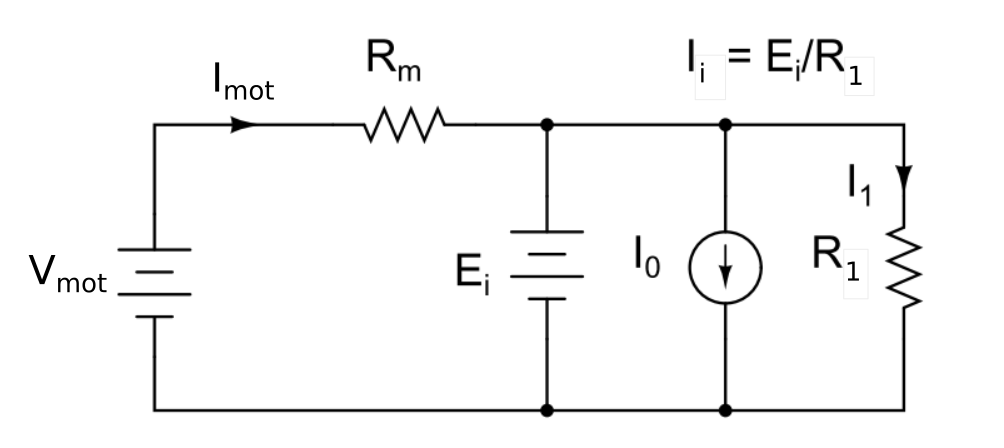
\includegraphics[width=0.7\textwidth]{figures/motor_electric_4c}
	\caption[Coefficient of Thrust as a function of Advance Ratio]{Coefficient of Thrust as a function of Advance Ratio}
	\label{fig:motor_electric_4c}
\end{figure}

The input to the motor is the driving voltage, $V_{mot}$ and the output is the output power, $P_{mot}$. Naturally, if there is a direct-drive configuration between the motor and the propeller, the motor rotational speed ($n_{mot}$, in revolutions per second) is the same as that of the propeller.

\begin{lstlisting}[style=C-style]
	n_prop = n_mot
\end{lstlisting}

\begin{IEEEeqnarray}{rCl}
	n_{mot} &= & K_v E_i \label{eq:motorKV}\\
	E_i &= & V_{mot} - I_{mot} R_m \label{eq:motorRM}\\
	P_{mot} &= & E_i I_i \\
	I_i &= & I_{mot} - I_0 - \frac{E_i}{R_1} \label{eq:motorR1}\\
	P_{elec} &= & V_{mot}I_{mot}
\end{IEEEeqnarray}

\begin{lstlisting}[style=C-style]
	n_mot = K_v*E_i
	E_i = V_mot - I_mot*R_m
	P_mot = E_i*I_i
	I_i = I_mot - I_0 - E_i/R_1
	P_elec = V_mot*I_mot
\end{lstlisting}

\subsection{Battery and Electronic Speed Controller}

Finally, an expression for the overall combination of the battery and ESC is given.
\begin{itemize}
\item $V_{bat}$ is the internal battery voltage
\item $R_{bat}$ is the battery internal resistance
\item $R_S$ is the ESC in-line resistance
\item $\delta_t$ is the throttle command, essentially modulating the output voltage
\end{itemize}

\begin{IEEEeqnarray}{rCl}
	V_{mot} &= & (V_{bat} - I_{mot} (R_{bat} + R_S)) \delta_t \label{eq:battR}
\end{IEEEeqnarray}

\begin{lstlisting}[style=C-style]
	V_mot = (V_bat - I_mot*(R_bat + R_S))*delta_t
\end{lstlisting}

%% IC engine model
\input{motor_ic}

